\documentclass[14pt]{extarticle}
\usepackage{amsmath}
\usepackage{amssymb}
%\usepackage{tikz}
%\usetikzlibrary{calc}
%\usetikzlibrary{trees}
\usepackage{hyperref}
\usepackage{graphicx}
\graphicspath{ {../../chap09/} }
\usepackage[top=0.75in, bottom=0.75in, left=0.75in, right=0.75in]{geometry}
%\newcommand*{\Scale}[2][4]{\scalebox{#1}{\ensuremath{#2}}}%
\usepackage[shortlabels]{enumitem}
\usepackage[most]{tcolorbox}
\definecolor{bg}{RGB}{255,249,227}
% \usepackage{showframe}
\title{\vspace{-5ex}Math 208 Section 9.5}
\date{\vspace{-10ex}}
%\usepackage{multicol}
%\setlength{\columnsep}{1cm}
\setlength{\parindent}{0pt}
\usepackage{parskip}
\setlength{\parskip}{10pt} % 1ex plus 0.5ex minus 0.2ex}
%\usepackage{ragged2e}


\begin{document}
	\maketitle		
	\section*{Homework, Reading, and Other}
	\begin{itemize}
		\item Section 9.4
		\item Section 9.5
	\end{itemize}

	\section{Goals}
	\begin{itemize}
		\item Comfortably use different derivative notations
		\item Recall and apply the Constant Rule, the Power Rule, the Constant Multiple Property, and the Sum and Difference Property.
		\item Refresh your proficiency when working with rational expressions, integer exponents, rational exponents, and algebraic manipulation of rational functions
	\end{itemize}
		

\section{Section 9.5: Differentiation}
\subsection{Introduction}
In Section 9.4, we defined the derivative and gave the four-step process for its determination. There are more notations that may be used with derivatives and you should be familiar with them.
\begin{center}
	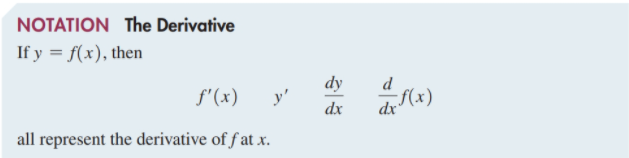
\includegraphics[width=0.9\linewidth]{9-5-1}
\end{center}
In this section, we will give a number of rules that make finding the derivative of a function much easier to find.

\subsection{Constant Rule}
\begin{center}
	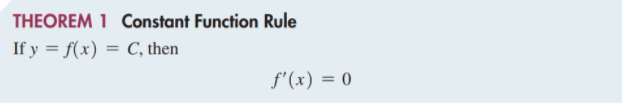
\includegraphics[width=0.9\linewidth]{9-5-2}
\end{center}
\subsubsection{Example}
If $f(x) = \pi * 4^2$, then
$$f'(x)= 0$$

\subsection{Power Rule}
\begin{center}
	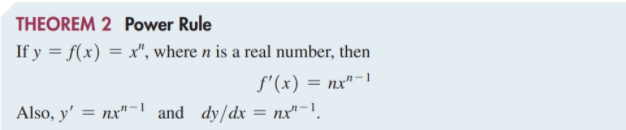
\includegraphics[width=0.9\linewidth]{9-5-3}
\end{center}
When using the power rule, have all powers in the numerator. Use your algebra skills to make the appropriate conversions. \textit{See Appendices A.4, A.5, and A.6} for a refresher.
\subsubsection{Examples}
\begin{itemize}
	\item If $y = x^3$, then
	$$y' = 3x^{3-1} = 3x^2$$
	\item If $y = \sqrt[3]{x} = x^{\frac{1}{3}}$, then
	$$ \frac{dy}{dx}= \frac{1}{3}x^{\frac{1}{3}-1}= \frac{1}{3}x^{-\frac{2}{3}}$$
	\item If $g(x) = \frac{1}{x^5} = x^{-5}$, then
	$$ \frac{d}{dx}g(x) = -5x^{-5-1} = -5x^{-6}$$
\end{itemize}

\subsection{Constant Multiple Property}
\begin{center}
	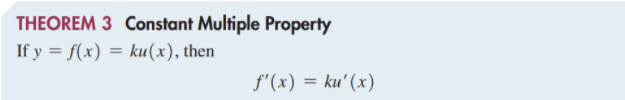
\includegraphics[width=0.9\linewidth]{9-5-4}
\end{center}
\subsubsection{Example}
If $h(x) = 4x^3$ then $$h'(x) = 4*3x^2 = 12x^2$$


\subsection{Sum and Difference Property}
\begin{center}
	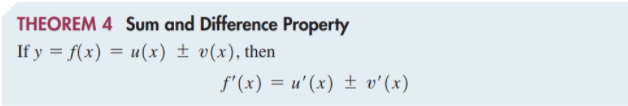
\includegraphics[width=0.9\linewidth]{9-5-5}
\end{center}
\subsubsection{Examples}
\begin{itemize}
	\item If $y = x^3 + x$, then
	$$y' = 3x^2+ 1$$
	\item If $g(x) = \frac{1}{\sqrt{x}} - 4x^2 = x^{-\frac{1}{2}} - 4x^2$, then
	$$ \frac{d}{dx}g(x) = -\frac{1}{2}x^{-\frac{3}{2}} - 8x$$
\end{itemize}

\subsection{Rewriting the function}
Often, you will need to rewrite the function using algebra before finding its derivative. We showed some examples earlier. ($\sqrt[3]{x} = x^{\frac{1}{3}}$, $\frac{1}{x^5} = x^{-5}$, and $\frac{1}{\sqrt{x}} = x^{-\frac{1}{2}}$) Here are two more standard methods.

Separate the fraction. Let
\begin{align*}
	f(x) &= \frac{3-x^3}{x^6} \\
	&= \frac{3}{x^6} - \frac{x^3}{x^6} \\
	&= 3x^{-6} - x{-3} \\\\
	f'(x) &= -18x^{-7} + 3x^{-4}
\end{align*}

Factor the fraction. Let
\begin{align*}
	g(x) & = \frac{x^2 +x -2}{x^2 -x} \\
	&= \frac{(x+2)(x-1)}{x(x-1)} \\
	&= \frac{x+2}{x} \\
	&= \frac{x}{x} + \frac{2}{x} \\
	&= 1 +2x^{-1} \\\\
	g'(x) & = -2x^{-2}
\end{align*}


\subsection{Application}
Say the velocity (in miles/hour) of a car is given by:
\begin{align*}
	v(t)=-\frac{13}{3}t^2 + 13t
\end{align*}
What is the maximum velocity of the car? (in other words, What is the maximum of this parabola?)

The key to this problem is to recognize that the slope of the tangent line at the maximum is equal to zero. Then set the derivative equal to zero to find the value of t at the maximum.
\begin{center}
	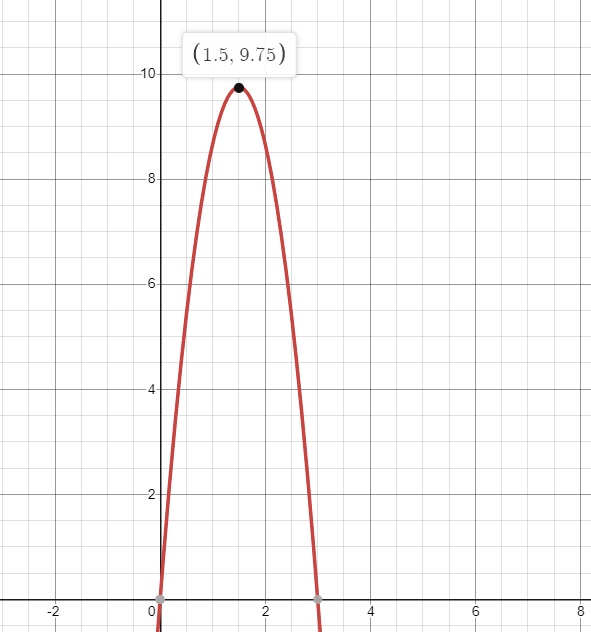
\includegraphics[width=0.6\linewidth]{9-5-20a}
\end{center}

\begin{align*}
	0 &= \frac{d}{dt}v(t) \\
	&=-\frac{26}{3}t + 13 \\
	\frac{26}{3}t &= 13 \\
	t &= \frac{39}{26} = \frac{3}{2}
\end{align*}
Finally, find the function value at $t = 3/2$.
\begin{align*}
	v\left(\frac{3}{2}\right) &= -\frac{13}{3}\left(\frac{3}{2}\right)^2 + 13\left(\frac{3}{2}\right) \\
	&= -\frac{13}{3}\left(\frac{9}{4}\right) + \frac{39}{2} \\
	& = \frac{39}{4} = 9.75
\end{align*}

\noindent\rule{\textwidth}{1pt}
{\footnotesize Copyright (C) 2021 Garold Dalton --- Released under GNU General Public License v3.0}


\cleardoublepage


\end{document}
